\section{Telepítőfájl létrehozása}

\begin{figure}
\centering
  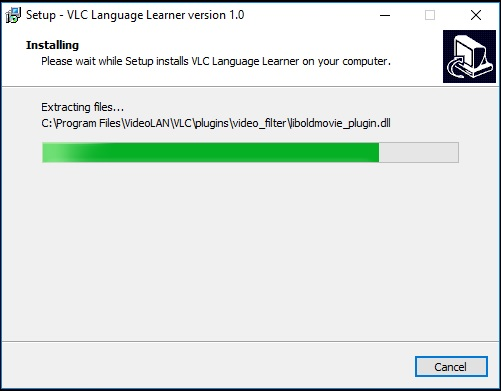
\includegraphics[width=.7\linewidth]{images/installer.jpg}
  \caption{Az alkalmazás telepítése}
  \label{fig:installer}
\end{figure}


Az alkalmazás elkészültével egy telepítőfájlt készítettem el, amely segítségével egyszerűen, gyorsan telepíthetőek a szükséges állományok bármely számítógépre. Jelenleg az alkalmazás csak 64 bites Windows operációs rendszerű számítógépeket támogat, melyhez egy telepítőfájl készült.

Először a \textit{.jar} fájl állítottam elő \textit{maven} segítségével. Ehhez a \textit{mvn package} parancsot kellett kiadjam a projekt könyvtárában. Ennek hatására a \textit{maven} a projekt fájljaiból előállított egy hordozható \textit{.jar} fájlt. A szoftver ezen formája azért nem elegendő számunkra, mert ahhoz, hogy az alkalmazás megfelelően működjön szükség van a \textit{VLC} könyvtárakra is, amelyeket a \textit{jar} nyilvánvalóan nem tartalmazza. Evégett hoztam létre egy telepítőt, amely minden szükséges könyvtárat feltelepít a felhasználó számítógépére.

Ehhez egy speciális alkalmazást használtam, melynek neve \textit{Inno Setup}. A szoftver képes a megadott fájlokból telepítővarázslót előállítani. Így bármely felhasználó néhány egyszerű kattintással telepítheti magának az alkalmazást. Ehhez először egy úgynevezett \textit{Inno Setup Script}-et kellett elkészítsek, amely alapján a szoftver a telepítőfájl összeállítását végzi. Itt szinte bármit megadhatunk, amely a telepítés folyamatát befolyásolja. A fájl nevét, verzióját, alapértelmezett telepítési könyvtárát. A megfelelő telepítő létrehozásához elengedhetetlen információt tartalmaz a \textit{Files} blokk. Itt kerülnek definiálásra azok a fájlok, amelyeket a telepítőszoftver összecsomagol (\ref{lst:files}). Ezen kívül ikon beállítására is van lehetőség, én a \textit{VLC} eredeti ikonjának kissé módosított változatát használtam.

\begin{lstlisting}[caption=Telepítőhöz szükséges fájlok, label={lst:files}]
[Files]
Source: "D:\workspace\VideoLAN\*";
   DestDir: "{app}";
   Flags: ignoreversion recursesubdirs createallsubdirs
Source: "D:\workspace\VideoLAN\basic-vlcj-1.0.jar";
   DestDir: "{app}";
   Flags: ignoreversion
Source: "D:\workspace\VideoLAN\icon.ico";
   DestDir: "{app}";
   Flags: ignoreversion;
\end{lstlisting}

A szkript összeállítása után a \textit{Run} gombra kattintva az \textit{Inno Setup} elkészíti a telepítőfájlt. Miután végzett megjelenik a telepítővarázsló, amely már az alkalmazásunk elkészült telepítője. Kiválaszthatjuk a telepítés helyét, amely alapértelmezetten a \textit{C:/Program Files/VideoLAN} könyvtár. Ezután a \textit{Next} gombra kattintva egy \textit{checkbox} segítségével kiválaszthatjuk, hogy szeretnénk-e az asztalon parancsikont létrehozni. Ismét kattintsunk a \textit{Next} gombra. Egy összesítő ablak jelenik meg, amelyen láthatjuk a telepítőben megadott útvonalat, illetve azt, hogy kiválasztottuk-e a parancsikon generálást. Amennyiben valamelyikkel nem értünk egyet, vagy esetleg rosszul adtuk meg az útvonalat, a \textit{Back} gombbal visszatérhetünk egészen a varázsló elejéhez. Ha mindennel egyetértünk, kattintsunk az \textit{Install} gombra. A telepítő elkezdi a szükséges fájlok megjelölt helyre történő másolását (\ref{fig:installer}). Miután végzett az alkalmazás indítható, az asztalon található parancsikon segítségével, amennyiben ezt kértük, vagy a telepítés helyén a \textit{VLC Language Learner.jar} fájlra történő dupla kattintással. Az alkalmazás bármikor törölhető a Windows \textit{Programok telepítése és törlése} menüpontban, illetve bármikor újratelepíthető az elkészült telepítőfájl segítségével. A telepítő működése jeleneleg csak Windows rendszeren, azon belül is 64 bites verzión biztosított.